\documentclass[a4paper,12pt]{article}

\usepackage{fontspec}
\setmainfont{Sora}
\usepackage[magyar]{babel}
\usepackage[hidelinks]{hyperref}
\usepackage{listings}
\usepackage{booktabs}
\usepackage{array}
\newcolumntype{L}[1]{>{\raggedright\arraybackslash}p{#1}}
\usepackage{graphicx}
\usepackage{xcolor}
\usepackage{fancyhdr}
\usepackage{tikz}
\usepackage{float}
\usepackage[left=2cm, right=2cm, top=3cm, bottom=6cm, footskip=2cm]{geometry}

% Brand colors
\definecolor{wosm-lila}{HTML}{604696}
\definecolor{szurke}{HTML}{aea8a6}

% Header
\pagestyle{fancy}
\fancyhf{}
\renewcommand{\headrulewidth}{0pt}
\fancyhead[L]{%
  \raisebox{-0.8cm}{%
    
\includegraphics[height=2cm]{csapat_logo_lila.png}%
    \hspace{0.4em}%
    {\color{szurke}\vrule width 0.8pt height 2cm}%
    \hspace{0.6em}%
    \vbox to 2cm{\vfill{\color{szurke}\bfseries\itshape\large 902.\\Kucsera Ferenc\\cserkészcsapat}\vfill}%
  }%
}
\setlength{\headheight}{2.5cm}
\setlength{\headsep}{1cm}

% Footer
\fancyfoot[L]{%
  \parbox{\textwidth}{\footnotesize\color{szurke}%
    \textbf{902. Kucsera Ferenc cserkészcsapat}\\
    szerző: Kerak\\
    fay.ambrus@cserkesz.hu}%
}
\fancyfoot[R]{\color{szurke}\thepage}

% Watermark
\usepackage{eso-pic}
\AddToShipoutPictureBG{%
  \AtPageLowerLeft{%
    \put(\dimexpr\paperwidth-7cm\relax,3cm){%
      \begin{tikzpicture}
        \node[opacity=0.06] {
\includegraphics[width=10cm]{csapat_logo_lila.png}};
      \end{tikzpicture}%
    }%
  }%
}

\title{\color{wosm-lila}\bfseries Pénzügyi tervező és nyilvántartó rendszer\\[0.3em]
  \large Rendszerspecifikáció}
\author{}
\date{}

\begin{document}
\maketitle
\thispagestyle{fancy}
\tableofcontents
\newpage

\section{Bevezetés}

A rendszer célja a 902. Kucsera Ferenc cserkészcsapat pénzügyi működésének támogatása.

\section{Követelmények}
\subsection{Felhasználói szerepkörök}
Ez az alszekció a rendszerben használt különböző felhasználói szerepeket részletezi. A különböző felhasználók, és a köztük lévő kapcsolatok az \ref{fig:users}. ábrán láthatóak. A követelményeknél fel fogjuk tüntetni, hogy melyik szerepkör jogosult az adott akció végrehajtására. Ezeken kívül lehetőség van részletesebb időkorlátos jogkör-bővítésre felhasználónként. A részletesebb jogkör-bővítést a \ref{sec:claims} szekció részletezi.
\begin{figure}
  \centering                                                                         
  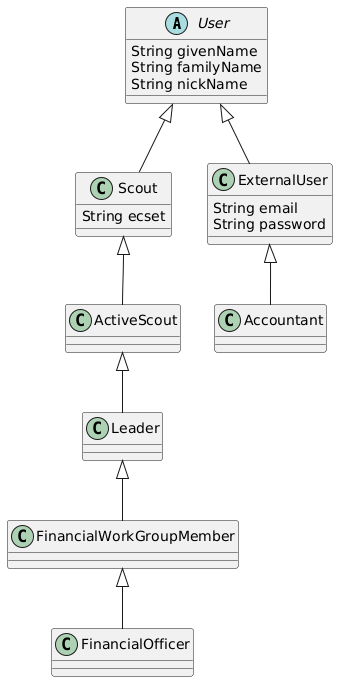
\includegraphics[width=0.55\textwidth]{diagrams/users-class-diagram.png}       
  \caption{Felhasználói osztálydiagram}\label{fig:users}                                                 
\end{figure}  
\subsubsection{Felhasználó}
Általános felhasználót reprezentáló típus. Önmagában semmilyen jogkörrel nem rendelkezik. Minden felhasználó esetében tároljuk a rendszerben a vezetéknevét, keresztnevét és opcionálisan a becenevét.
\subsubsection{Cserkész}
Felhasználótípus, ami a Magyar Cserkészszövetség azon tagjait reprezentálja, akik a 902. Kucsera Ferenc cserkészcsapat tagjai. Minden cserkész rendelkezik ECSET-kóddal. A cserkész felhasználók csak ECSET-en keresztül jelentkezhetnek be a rendszerbe.
\subsubsection{Aktív cserkész}
Felhasználótípus, ami azon cserkészeket reprezentálja, akik ECSET-ben aktív státusszal rendelkeznek.
\subsubsection{Vezető}
Felhasználótípus, ami azon aktív cserkészeket reprezentálja, akik ECSET-ben rendlekeznek valamilyen csapaton belüli megbiízatással, vagy munkacsoport-tagok.
\subsubsection{Pénzügyi munkacsoport-tag}
Felhasználótípus, ami azon vezetőket reprezentálja, akik tagjai a pénzügyi munkacsoportnak.
\subsubsection{Pénzügyi vezető}
Felhasználótípus, ami azon vezetőket reprezentálja, akik "teljes", vagy "pénzügyes" szintű megbizatással rendelkeznek ECSET-ben a csapaton.
\subsubsection{Külső felhasználó}
Azon felhasználókat reprezentálja, akik nem tagjai a csapatnak, de mégis valamilyen hozzáférésük van a rendszerhez. Számukra az ECSET-en keresztüli bejelentkezés helyett email-címmel és jelszóval történő bejelentkezés elérhető. A rendszer tárolja az emailcímüket és jelszavukat. Ilyen felhasználó tipikusan egy olyan szülő, aki külsősként részt vesz egy programon segítőként.
\subsubsection{Könyvelő}
A csapat könyvelőjét reprezentáló felhasználótípus.
\subsection{Alapfogalmak}
\subsubsection{Összeg}
Valaemennyi pénzösszeget jelez. Részei
\begin{itemize}
  \item pénz
  \item pénznem (forint, euró, dollár stb.)
\end{itemize}
\subsubsection{Banki tranzakció}
Egy banki tranzakció reprezentálása a rendszerben. A következő részekkel rendelkezik:
\begin{itemize}
  \item értéknap
  \item partner neve
  \item partner számlaszáma
  \item összeg (forint)
  \item közlemény
  \item projekt
  \item megjegyzés
\end{itemize}
\subsubsection{Készpénzed tranzakció}
Egy készpénzes tranzakció reprezentálása a rendszerben. A következő részekkel rendelkezik:
\begin{itemize}
  \item értéknap
  \item partner neve
  \item összeg
  \item közlemény
  \item projekt
  \item megjegyzés
\end{itemize}
\subsubsection{Projekt}
Egy pénzügyi projekt egy meghatározott cél elérésére irányuló határidő-, költség-, erőforráskorlátokkal rendelkező, megtervezett és végrehajtott tevékenységsorozat, amely konkrét célokat valósít meg. Projekt például egy csapatprogram, a Stéger egy évi fejlesztése vagy akár egy őrs/raj fenntartása is egy projekt. A projektekhez tranzakciók rendelhetőek és minden tranzakció kötelezően pontosan egy projekthez tartozik. A projektek a következő részekkel rendelkeznek:
\begin{itemize}
  \item név
  \item leírás (opcionális)
  \item pénzügyi felelős
  \item tranzakciók
  \item pénzügyi terv (opcionális)
  \item beszámoló
  \item kezdő- és befejező dátum
  \item státusz: létrhozva, terv beadva, terv elfogadva, projekt vége, beszámoló elfogadva
\end{itemize}


\subsection{Funkcionális követelmények}
\subsubsection{Banki tranzakciók betöltése}
\begin{table}[H]
  \centering
  \begin{tabular}{llL{8cm}l}
  \toprule
  Azonosító & Szerepkör & Leírás & Prioritás \\
  \midrule
  FR-a01 & Rendszer         & Naponta háromszor letöltödnek a banki tranzakciós adatok a GoCardless API-ját használva.  & Magas \\
  FR-a02 & Pénzügyi vezető  & Csapathoz tartozó bankszámlák rögzítése, olvasása és törlése. (IBAN formátumban)          & Magas \\
  FR-a03 & Pénzügyi vezető  & A rendszerben szereplő bankkártyákhoz GoCardless kapcsolat létrehozása.                   & Magas \\
  FR-a04 & Vezető           & A betöltött tranzakciók megtekintése. (Duplikátumok nélkül.)                              & Magas \\
  FR-a05 & Pénzügyi mcsp.   & A betöltött tranzakciók jelölése duplikátumként.                                          & Magas \\
  FR-a06 & Vezető           & Tranzakciók feldarabolása több részre.                                                    & Magas \\
  FR-a07 & Vezető           & Tranzakciók nyitott projektekhez rendelése.                                               & Magas \\
  \bottomrule
  \end{tabular}
\end{table}

\subsubsection{Projektek}
\begin{table}[H]
  \centering
  \begin{tabular}{llL{8cm}l}
  \toprule
  Azonosító & Szerepkör & Leírás & Prioritás \\
  \midrule
  FR-b01 & Vezető           & Projektek létrehozása és olvasása.                                                        & Magas \\
  FR-b02 & Vezető           & Saját projektek módosítása és törlése.                                                    & Magas \\
  FR-b03 & Pénzügyi mcsp.   & Minden projekt módosítása és törlése.                                                     & Magas \\
  FR-b04 & Vezető           & Közlemény-kifejezésel létrehozása, olvasása, módosítása, törlése.                         & Magas \\
  FR-b04 & Rendszer         & Közlemény-kifejezésel létrehozása, olvasása, módosítása, törlése.                         & Magas \\
  \bottomrule
  \end{tabular}
\end{table}
\subsection{Nem-funkcionális követelmények}

\section{Technológiai környezet}
% .NET 10, ASP.NET Core Web API, EF Core, SQLite, OpenAPI

%\section{Hitelesítés és jogosultságkezelés}
%\subsection{Lokális bejelentkezés (Identity)}
%\subsection{OIDC bejelentkezés (ecset.cserkesz.hu)}
%\subsubsection{Tokenek és scope-ok}
%\subsubsection{Felhasznált claim-ek}
%\label{sec:claims}
%\subsection{Jogosultsági szintek}

%\section{Tartománymodell}
%\subsection{Személyek}
%% Person, Scout, Administrator, Accountant, Family
%\subsection{Szervezeti egységek (Unit)}
%% Őrs, raj, csapat, munkacsoport; hierarchia
%\subsection{Pénzügyek}
%\subsubsection{Transaction}
%\subsubsection{BankAccount}
%\subsubsection{TransactionPartner és ITransactable}
%\subsubsection{Money (értéktípus)}
%\subsection{Pénzügyi tervezés}
%\subsubsection{FinancialProject}
%\subsubsection{FinancialPlan}
%\subsubsection{PlanItem és formulák}
%\subsubsection{PlanParameter}
%\subsection{Események (Event)}
%\subsection{Enumerációk}
%
%\section{API terv}
%\subsection{Konvenciók}
%% Controller routing, JSON, OpenAPI
%\subsection{Auth végpontok}
%\subsection{Személy végpontok}
%\subsection{Szervezeti egység végpontok}
%\subsection{Tranzakció végpontok}
%\subsection{Pénzügyi terv végpontok}
%\subsection{Esemény végpontok}
%
%\section{Adatbázis}
%\subsection{EF Core leképezés}
%% TPH öröklés, Owned type (Money), self-referencing Unit
%\subsection{Migrációk}
%
%\section{Pénzügyi terv kiértékelése}
%% Frontend: expr-eval, backend: opaque string + resolved érték
%% Opcionális backend kiértékelés: DynamicExpresso
%
%\section{Fejlesztési környezet}
%\subsection{Futtatás és portok}
%\subsection{Titkos kulcsok kezelése (.NET User Secrets)}
%
%\section{Tesztelés}
%
%\section{Telepítés és üzemeltetés}
%
%\section{Továbbfejlesztési lehetőségek}

\end{document}
